% **************************************************
% Clean Thesis
% -- A LaTeX Style for Thesis Documents --
%
% Copyright (C) 2011-2015 Ricardo Langner
% **************************************************
%
% Readme:
% ----------------------------------------
% Please check out the README.md file in the root of this package.
%
%
% License Information:
% ----------------------------------------
% "Clean Thesis" is free software: you can redistribute it and/or modify
% it under the terms of the GNU General Public License as published by
% the Free Software Foundation, either version 3 of the License, or
% (at your option) any later version.
%
% "Clean Thesis" is distributed in the hope that it will be useful,
% but WITHOUT ANY WARRANTY; without even the implied warranty of
% MERCHANTABILITY or FITNESS FOR A PARTICULAR PURPOSE.  See the
% GNU General Public License for more details.
%
% You should have received a copy of the GNU General Public License
% along with this program.  If not, see <http://www.gnu.org/licenses/>.
% **************************************************


% **************************************************
% Document Class Definition
% **************************************************
\documentclass[%
	paper=A4,					% paper size --> A4 is default in Germany
	twoside=true,				% onesite or twoside printing
	openright,					% doublepage cleaning ends up right side
	parskip=full,				% spacing value / method for paragraphs
	chapterprefix=true,			% prefix for chapter marks
	11pt,						% font size
	headings=normal,			% size of headings
	bibliography=totoc,			% include bib in toc
	listof=totoc,				% include listof entries in toc
	titlepage=on,				% own page for each title page
	captions=tableabove,		% display table captions above the float env
	draft=false,				% value for draft version
]{scrreprt}%

% **************************************************
% Debug LaTeX Information
% **************************************************
%\listfiles

% **************************************************
% Information and Commands for Reuse
% **************************************************
\newcommand{\thesisTitle}{High energy phenomena: A window to the dark universe.}
\newcommand{\thesisName}{Jonatan Selsing}
\newcommand{\thesisSubject}{Part A Thesis}
\newcommand{\thesisDate}{August 22, 2015}
\newcommand{\thesisVersion}{0.1}

\newcommand{\thesisFirstReviewer}{Dr. Lise Christensen}
\newcommand{\thesisFirstReviewerDepartment}{\protect{Dark Cosmology Centre}}
\newcommand{\thesisFirstReviewerUniversity}{Niels Bohr Institute, University of Copenhagen}

\newcommand{\thesisSecondReviewer}{Dr. Maximilian Stritzinger}
\newcommand{\thesisSecondReviewerUniversity}{\protect{Aarhus University}}
\newcommand{\thesisSecondReviewerDepartment}{Department of Physics and Astronomy}

\newcommand{\thesisFirstSupervisor}{Dr. Lise Christensen}
\newcommand{\thesisSecondSupervisor}{}

\newcommand{\thesisUniversity}{\protect{University of Copenhagen}}
%\newcommand{\thesisUniversityDepartment}{}
\newcommand{\thesisUniversityInstitute}{Niels Bohr Institute}
\newcommand{\thesisUniversityGroup}{Dark Cosmology Centre (DARK)}
\newcommand{\thesisUniversityCity}{Copenhagen}
\newcommand{\thesisUniversityStreetAddress}{Juliane Maries Vej 30}
\newcommand{\thesisUniversityPostalCode}{2100 Copenhagen Ø}

% **************************************************
% Load and Configure Packages
% **************************************************
\usepackage[utf8]{inputenc}		% defines file's character encoding

\usepackage{newunicodechar}
\newunicodechar{‐}{-}
%\newunicodechar{}{-}


\usepackage[english]{babel} % babel system, adjust the language of the content
\usepackage[					% clean thesis style
	figuresep=colon,%
	sansserif=false,%
	hangfigurecaption=false,%
	hangsection=true,%
	hangsubsection=true,%
	colorize=full,%
	colortheme=bluemagenta,%
	bibsys=bibtex,%
	bibfile=/Users/jselsing/Work/Papers/bibtex/library.bib,%
	bibstyle=authoryear,%
]{cleanthesis}


\hypersetup{					% setup the hyperref-package options
	pdftitle={\thesisTitle},	% 	- title (PDF meta)
	pdfsubject={\thesisSubject},% 	- subject (PDF meta)
	pdfauthor={\thesisName},	% 	- author (PDF meta)
	plainpages=false,			% 	-
	colorlinks=true,			% 	- colorize links?
	linkcolor=[cmyk]{1.0, 0.50, 0.10, 0.01},
%	linkcolor=[cmyk]{.18, .98, .18, 0},
	pdfborder={0 0 0},			% 	-
	breaklinks=true,			% 	- allow line break inside links
	bookmarksnumbered=true,		%
	bookmarksopen=true			%
}

\AtEveryBibitem{\clearfield{title}}
\AtEveryBibitem{\clearfield{eprint}}



\DeclareFieldFormat{citehyperref}{%
  \DeclareFieldAlias{bibhyperref}{noformat}% Avoid nested links
  \bibhyperref{#1}}

\DeclareFieldFormat{textcitehyperref}{%
  \DeclareFieldAlias{bibhyperref}{noformat}% Avoid nested links
  \bibhyperref{%
    #1%
    \ifbool{cbx:parens}
      {\bibcloseparen\global\boolfalse{cbx:parens}}
      {}}}

\savebibmacro{cite}
\savebibmacro{textcite}

\renewbibmacro*{cite}{%
  \printtext[citehyperref]{%
    \restorebibmacro{cite}%
    \usebibmacro{cite}}}

\renewbibmacro*{textcite}{%
  \ifboolexpr{
    ( not test {\iffieldundef{prenote}} and
      test {\ifnumequal{\value{citecount}}{1}} )
    or
    ( not test {\iffieldundef{postnote}} and
      test {\ifnumequal{\value{citecount}}{\value{citetotal}}} )
  }
    {\DeclareFieldAlias{textcitehyperref}{noformat}}
    {}%
  \printtext[textcitehyperref]{%
    \restorebibmacro{textcite}%
    \usebibmacro{textcite}}}

\renewcommand{\baselinestretch}{1.2}
\setlength{\parskip}{\smallskipamount}
\setlength{\parindent}{0pt}



% **************************************************
% Document CONTENT
% **************************************************
\begin{document}

% --------------------------
% rename document parts
% --------------------------
%\renewcaptionname{ngerman}{\figurename}{Abb.}
%\renewcaptionname{ngerman}{\tablename}{Tab.}
\renewcaptionname{english}{\figurename}{Fig.}
\renewcaptionname{english}{\tablename}{Tab.}

% --------------------------
% Front matter
% --------------------------
\pagenumbering{roman}			% roman page numbing (invisible for empty page style)
\pagestyle{empty}				% no header or footers
% !TEX root = ../thesis-example.tex
%
% ------------------------------------  --> cover title page
\begin{titlepage}
	\pdfbookmark[0]{Cover}{Cover}
	\flushright
	\hfill
	\vfill
	{\LARGE\thesisTitle \par}
	\rule[5pt]{\textwidth}{.4pt} \par
	{\Large\thesisName}
	\vfill
	\textit{\large\thesisDate} \\
	Version: \thesisVersion
\end{titlepage}


% ------------------------------------  --> main title page
\begin{titlepage}
	\pdfbookmark[0]{Titlepage}{Titlepage}
	\tgherosfont
	\centering

	{\Large \thesisUniversity} \\[4mm]
	
\includegraphics[width=10cm]{gfx/dark3} \\[2mm]
%	\textsf{\thesisUniversityDepartment} \\
	\textsf{\thesisUniversityInstitute} \\
	\textsf{\thesisUniversityGroup} \\

	\vfill
	{\large \thesisSubject} \\[5mm]
	{\LARGE \color{ctcolortitle}\textbf{\thesisTitle} \\[10mm]}
	{\Large \thesisName} \\

	\vfill
	\begin{minipage}[t]{.27\textwidth}
		\raggedleft
		\textit{1. Reviewer}
	\end{minipage}
	\hspace*{15pt}
	\begin{minipage}[t]{.65\textwidth}
		{\Large \thesisFirstReviewer} \\
	  	{\small \thesisFirstReviewerDepartment} \\[-1mm]
		{\small \thesisFirstReviewerUniversity}
	\end{minipage} \\[5mm]
	\begin{minipage}[t]{.27\textwidth}
		\raggedleft
		\textit{2. Reviewer}
	\end{minipage}
	\hspace*{15pt}
	\begin{minipage}[t]{.65\textwidth}
		{\Large \thesisSecondReviewer} \\
	  	{\small \thesisSecondReviewerDepartment} \\[-1mm]
		{\small \thesisSecondReviewerUniversity}
	\end{minipage} \\[10mm]
	\begin{minipage}[t]{.27\textwidth}
		\raggedleft
		\textit{Supervisor}
	\end{minipage}
	\hspace*{15pt}
	\begin{minipage}[t]{.65\textwidth}
		\thesisFirstSupervisor\ 
	\end{minipage} \\[10mm]

	\thesisDate \\

\end{titlepage}


% ------------------------------------  --> lower title back for single page layout
\hfill
\vfill
{
	\small
	\textbf{\thesisName} \\
	\textit{\thesisTitle} \\
	\thesisSubject, \thesisDate \\
	Reviewers: \thesisFirstReviewer\ and \thesisSecondReviewer \\
	Supervisor: \thesisFirstSupervisor\  \\[1.5em]
	\textbf{\thesisUniversity} \\
	\textit{\thesisUniversityGroup} \\
	\thesisUniversityInstitute \\
%	\thesisUniversityDepartment \\
	\thesisUniversityStreetAddress \\
	\thesisUniversityPostalCode\ and \thesisUniversityCity
}
		% INCLUDE: all titlepages
%\cleardoublepage

\pagestyle{plain}				% display just page numbers
% !TEX root = Clean-Thesis.tex
%
\pdfbookmark[0]{Abstract}{Abstract}
\chapter*{Abstract}
\label{sec:abstract}
\vspace*{-10mm}

Because of the vast expanse of the universe we live in, very little starlight reaches us from the environments furthest from us. To explore the region of space unavailable to us via direct detection, extremely energetic phenomena can be used to investigate the space between us and them, by illuminating the universe otherwise obscured. Gaining a thorough understanding of the physical processes at play in the high-energy events populating our universe is of prime importance because any signatures deviating from the intrinsic appearance of the object can be attributed to the intervening material and thus an indirect inference can be made about the dark universe. In this thesis I present some of the work I am involved with related to high-energy phenomena, specifically: Quasars (QSOs), Gamma-Ray Bursts (GRBs) and Supernovae (SNe). The work I present here consists of four projects I am involved with and the majority is still a work in progress where additional work is need before publication. The work I have been doing is specifically the \textit{average} properties of the UV to near-infrared spectra of a selection of QSOs, the explosion environments of high-velocity ejecta core-collapse supernovae, the average optical afterglow of long-duration GRBs and the search for high-redshift, lensed SNe, including the quadruply lensed "SN Refsdal".




		% INCLUDE: the abstracts (english and german)
\clearpage
%
%% !TEX root = ../thesis-example.tex
%
\pdfbookmark[0]{Acknowledgement}{Acknowledgement}
\chapter*{Acknowledgement}
\label{sec:acknowledgement}
\vspace*{-10mm}

\Blindtext[2][2]
 % INCLUDE: acknowledgement
%\cleardoublepage
%
\setcounter{tocdepth}{2}		% define depth of toc
\tableofcontents				% display table of contents
%\cleardoublepage

% --------------------------
% Body matter
% --------------------------
\pagenumbering{arabic}			% arabic page numbering
\setcounter{page}{1}			% set page counter
\pagestyle{maincontentstyle} 	% fancy header and footer

% !TEX root = ../thesis-example.tex
%
\chapter{High-energy space phenomena: A window to the dark universe.}
\section{Introduction}
\label{sec:intro}

\cleanchapterquote{Astronomy? Impossible to understand and madness to investigate.}{Sophocles (450 BC)}{} \\

In this Part A Thesis I will summarize some of the work I have been doing during
the
first two years of my PhD, while also officially enrolled in the masters
programme. The work I have done is mainly divided into three subjects: QSOs,
GRBs and SNe and is related to various aspects of the different subjects. 

For QSOs, I have researched the average properties of a sample of bright $M_{r}
\leq -27.5$ QSOs and created a composite spectrum for community usage. I showed
an application of the composite in inferring dust content of the quasar host
galaxies and additionally, I find a steeper slope of the quasar power-law
continuum
as compared to the traditionally assumed one, indicating an
intrinsically harder
continuum. This project therefore investigates both
intrinsic properties of the
quasar phenomena, but also allows for the conditions
of the intervening material to be
inferred, both in the quasar host or potential
absorption systems in the
line-of-sight.

For GRBs, I am involved with the X-shooter GRB collaboration and will be
investigating the average properties of the GRB optical afterglows for the
sample we are building. Data-collection for the sample is continuous and we have
an ESO TOO-program to do ground-based follow-up of the optical afterglow from
GRBs detected with \textit{Swift}.  I have developed an algorithm to normalize
the afterglows, which is then used  as a product of the afterglow sample, for
example for absorption-line studies. Once a sufficient sample size is
reached, I will lead a project to construct a composite afterglow spectrum. This
afterglow composite can then be used twofold: as a cross-correlation template to
determine redshift for newly discovered noisy afterglows and as a way to
explore
the average properties of the optical afterglows, thereby also allowing
identification of potentially interesting outliers for further observations. 

For SNe, I am involved in two projects. One related to the explosion
environments of type Ic and Ic-BL supernovae without accompanying GRBs where we
have obtained a sample of 19 supernova host galaxies observed with an IFU,
allowing spatially resolved diagnostics to be calculated for the stellar
progenitor population. This work is done to investigate whether the explosion
environments of the
two types of SNe differ and can also be used to constrain
the explosion
mechanisms for the different kinds of SNe. This project is in an
indirect way
related to an investigation of the GRB progenitor system, because
fast-ejecta
SNe are sometimes seen associated with GRBs and the reason why some
GRBs have
SNe and others don't remains a mystery. The other SN-project I am
involved with is a collaboration with the Frontier Fields program, where
spectroscopic follow-up of potential high-redshift supernovae are carried out
using X-shooter. The scientific rationale behind this project is the increased
chance of "serendipitously" discovering high-redshift SN in the Frontier Fields
because of the strong gravitational lensing in the galaxy clusters targeted. If
high-redshift SN are of the Ia-type this will help constrain our current
cosmology where the high-redshift SNe carry the highest leverage in terms of
discerning between different world-models. As part of this work I am working on
the quadruply lensed supernova "SN Refsdal" where the X-shooter observations
have helped constrain the SN type.

This report will present a brief status of the work that has been done in the
three fields and how it relates this to my own research. Apart from the research
I have been doing, I have taken 31 ECTS points distributed in the following
PhD-schools and regular courses: "Coping with the challengers of a PhD +
Scientific Writing", "Responsible Conduct of Research", "Introduction to
University Pedagogy", "Summer Schools in Statistics and Computation for
Astronomers", "Introduction to sub-mm interferometry and science with ALMA",
"Advanced Methods in statistical data analysis", "Classical Astrophysical
Papers". Additionally I have taught the mandatory 840 hours including the
Mechanics 1 and 2
courses for which I was awarded the Jens-Martin prize for
excellence in
teaching.

I will conclude with an outlook of what I will be working on in the last two
years of my PhD. 
I attach the submitted quasar paper, and the advanced draft of
the "SN Refdal"-paper with this Part A Thesis.


\clearpage

{\Large Publications} \\
{\large Paper I} \\
\textit{An X-shooter composite of bright $1<z<2$ quasars from UV to Infrared} \\
\textbf{Selsing, J}; Fynbo, J. P. U.; Christensen, L;  Krogager, J.-K. \\
\textit{Submitted to A\&A. Recommended for publication after minor revision.} \\

{\large Paper II} \\
\textit{Spectroscopic classification and confirmation of the first multiply imaged supernova}\\
P. L. Kelly, G. Brammer, \textbf{J. Selsing}, S. A. Rodney, J. Hjorth, R. J. Foley, L Christensen, and et al. \\
\textit{Advanced draft} \\


{\large Paper III} \\
\textit{Spectrophotometric analysis of GRB afterglow extinction curves with X-shooter} \\
J. Japelj, S. Covino, A. Gomboc, S. D. Vergani, P. Goldoni,\textbf{ J. Selsing}, Z. Cano, V. D'Elia, H. Flores, J. P. U. Fynbo, F. Hammer, J. Hjorth, P. Jakobsson, L. Kaper, D. Kopač, T. Krühler, A. Melandri, S. Piranomonte, R. Sánchez-Ramírez, G. Tagliaferri, N. R. Tanvir, A. de Ugarte Postigo, D. Watson, R. A. M. J. Wijers \\
\citet{Japelj2015} \\


{\large Paper IV} \\
\textit{GRB hosts through cosmic time - VLT/X-shooter emission-line spectroscopy of 96 GRB-selected galaxies at 0.1 < z < 3.6} \\
T. Krühler, D. Malesani, J. P. U. Fynbo, O. E. Hartoog, J. Hjorth, P. Jakobsson, D. A. Perley, A. Rossi, P. Schady, S. Schulze, N. R. Tanvir, S. D. Vergani, K. Wiersema, P. M. J. Afonso, J. Bolmer, Z. Cano, S. Covino, V. D'Elia, A. de Ugarte Postigo, R. Filgas, M. Friis, J. F. Graham, J. Greiner, P. Goldoni, A. Gomboc, F. Hammer, J. Japelj, D. A. Kann, L. Kaper, S. Klose, A. J. Levan, G. Leloudas, B. Milvang-Jensen, A. Nicuesa Guelbenzu, E. Palazzi, E. Pian, S. Piranomonte, R. Sanchez-Ramirez, S. Savaglio, \textbf{J. Selsing}, G. Tagliaferri, P. M. Vreeswijk, D. J. Watson, D. Xu \\
\citet{Kruhler2015} \\

\clearpage


\section{Quasars: Cosmic Lighthouses}
\label{sec:intro:qso}

The word quasar is derived from quasi-stellar radio source which is what
quasars
were initially detected as: point-like radio sources without an optical
counterpart. When the first optical counterpart was discovered it indeed
resembled a blue star, but spectroscopic follow-up revealed a confusing pattern
with very broad emission lines superposed on a blue continuum. When the lines
were matched to the correct atomic species, a cosmological origin was
established which posed a problem for the mechanisms powering the source because
the extreme energies inferred. The Eddington limit is the maximal luminosity a
gravitationally bound object of a given mass can have without radiation pressure
tearing the object apart and at the luminosities inferred from the cosmological
origin of the quasars and the observed brightness’s the required masses of the
sources were extremely high. Quasars also exhibits a large
degree of variability
in the observed flux on differing time-scales in the order
of weeks and years
with shorter time-scale variability is superposed on longer
variability periods.
The short timescale variability observed require a relatively small
emitting
regions, which poses a problem for a potential stellar origin of the
emission
and gives merit to the idea of a black hole powering the emission.
One of the
first quasars discovered, 3C 273, is estimated
to have a mass of $\sim900 \times
10^{6} M_\odot$ \citep{Peterson2004}
determined using a technique called
reverberation mapping in which the
time-delay between the continuum emission and
line emission is used to infer the
radius of the emitting region. From the
radius of the emitting region and the
velocity of the emitting material, an
estimate of the gravitational mass can be
made. The mass inferred for 3C 273 far
exceeds the maximal possible mass a star
can have before it would immediately
collapse to a back hole \citep{Belczynski2010}.


The optical-to-ultraviolet emission mechanism of quasars is by now quite well
understood \citep{Elvis1994}. A supermassive black hole at the center of a
galaxy is surrounded by a hot accretion disc, which emits a featureless thermal
continuum \citep{Shakura1973, Pereyra2006}. The central continuum photoionizes a
region of hot clouds, and further out, cold clouds which gives rise to lines
with both broad and narrow components \citep{Elvis2001}.  Varying conditions in
the clouds ensure that each ionic species have optimal conditions to produce
line emission \citep{Baldwin1995}. Despite the apparent different conditions in
which the emission arises, the overall shape of most quasar spectra looks
similar
\citep{Dietrich2002}. The remarkable uniformity of the average spectral
properties across luminosity and redshift indicate very similar underlying
physical mechanisms which can be understood in terms of Eigenvector 1
\citep{Boroson1992, Francis1992} where the Eddington ratio drives the relative
strength of the lines and orientation effects influences the observed kinematics
of the lines \citep{Shen2014a} accounting for the majority of the inter-quasar
variation. This means that the accretion rate and the mass of the black hole
largely determine the spectral appearance of a given quasar. Quasars are a part
of a more general class of objects called Active Galactic Nuclei (AGN) and the
classification of a given type
is in part believed to be viewing effects
\citep{Elvis2001}.


The average quasar spectrum of the sample presented in Paper I is shown in Fig.\,\ref{fig:intro:qsospec} where the position of the most prominent emission lines
has been marked. The purple dashed line is a power-law fit to the spectral regions
deemed free of contaminating emission lines and it can be seen that a pure
power-law relatively well describes the continuum, which is also the shape that
is predicted from \citet{Pereyra2006}.

\begin{figure}[htb]
	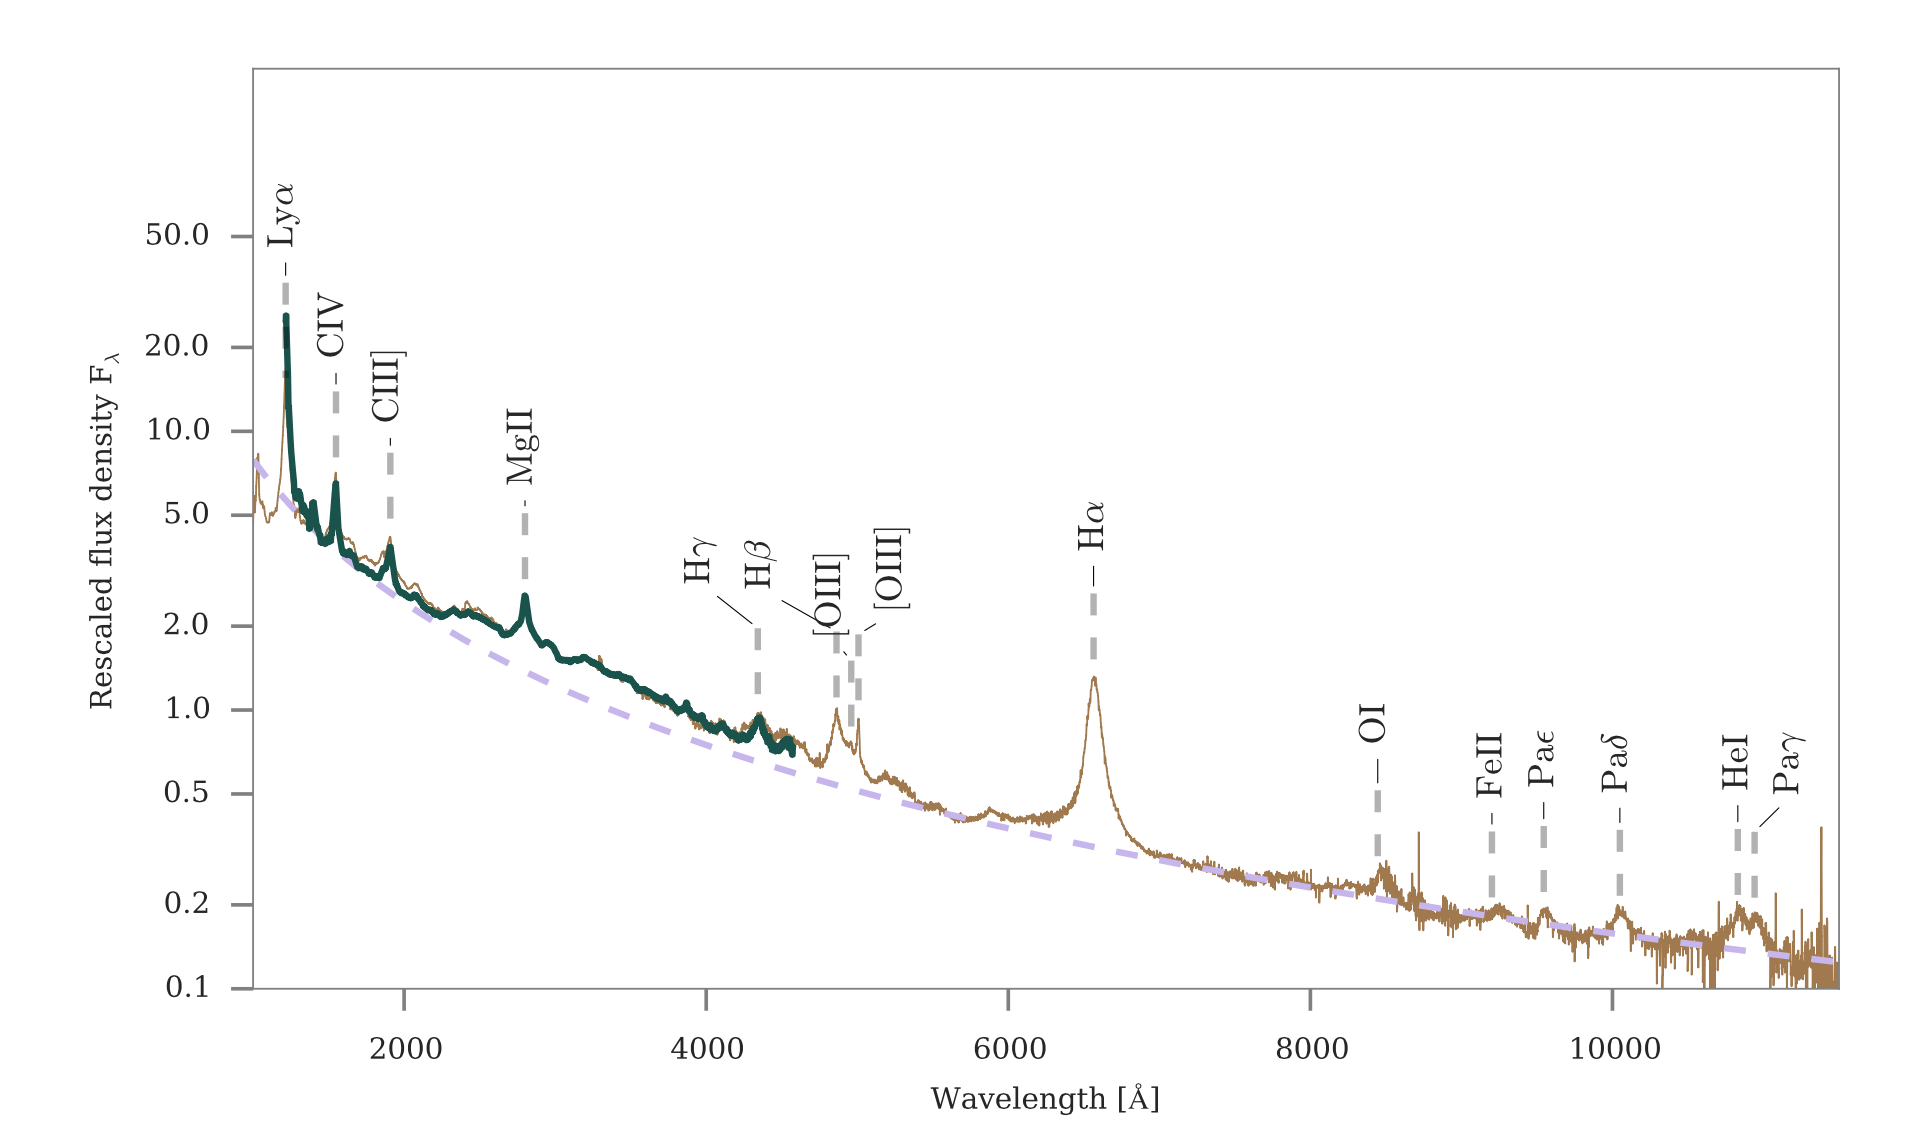
\includegraphics[width=\textwidth]{gfx/qsospec}
	\caption{Quasar composite spectrum from Paper I. The brown line is the average
quasar spectrum where several of the prominent lines have been marked. The purple
dashed line is a power-law fit to the regions free of contaminating emission and
 the dark green line is an average spectrum constructed for all SDSS spectra
fulfilling the selection criteria imposed on the sample observed with
X-shooter.}
	
	\label{fig:intro:qsospec}
\end{figure}


Even though the general principles behind the quasar phenomena seems to be
relatively well understood, important details remains unknown especially in
terms of
understanding the total contribution of the quasar feedback in
regulating star
formation in galaxies \citep{DiMatteo2005}, how the first quasar
became so
massive so rapidly after the creating of the universe \citep{Wu2015a},
how the
co-evolution of the quasars and their host galaxies works
\citep{Ferrarese2000},
what role quasars played in reionization
\citep{Hopkins2007} and what shape the intrinsic optical/ultraviolet (UV)
spectral energy distribution has \citep{Krawczyk2015}. The quasar contribution
to
reionization depends on the quasar luminosity function (QLF), which in turn
depends on the assumed slope of the quasar SED. The QLF is the integrated
luminosity of all quasars as a function of redshift and when calculating it, a
representative quasar SED model is required. The quasar optical SED is usually
is modeled by a power-law where the slope of the quasar continuum is determined
from the average slope of large samples of quasars \citep{Vandenberk2001,
Richards2006a, Shen2011, Lusso2015} where regions free of emission lines is
determined "by-hand". It is very efficient to build large samples of quasars
from SDSS \citep{Paris2014}, but the relatively modest wavelength coverage of
the instrument install at Apache Point Observatory \citep{Gunn2006} makes it
difficult to uniquely determine a representative slope. Work has been done to
extend the average quasar spectrum to longer wavelengths using other instruments
\citep{Glikman2006}, but a well-defined sample of quasars with spectra covering
the entire range from ultra-violet to near infrared has not been compiled.
The
work I have carried out in Paper I seeks to address specifically this point
by
observing 7 extremely bright, $M_{r} \leq -27.5$, quasars which will
therefore
contain negligible amounts of host galaxy contamination. Additionally
the
composite spectrum I have generated can be used to infer the dust content of
the
quasar host galaxy and potential intervening absorption systems,
specifically
Damped Lyman Alpha (DLA) systems. DLAs are defined as having
hydrogen column
densities higher than $N_{\mathrm{HI}} > 2 \times 10^{20}
cm^{-2}$, determined
from the equivalent width of the hydrogen absorption lines or absorption line
profile fitting.
This class of objects are believed to be self-shielding systems
of gas that
contain a significant fraction of the neutral hydrogen at redshift
$z \sim 5$
\citep{StorrieLombardi2000}. Since these objects are to a large
degree observed in
absorption, our understanding of these object depend heavily
on our knowledge of
the illuminating object. An example of inferring the dust
properties and amount
is presented in \citet{Krogager2015}, where artificially
reddening a composite quasar
spectrum is used to fit for the amount of dust
under some assumed extinction
law. The quasar composite used in that work
consists of the template by
\citet{Vandenberk2001} stitched together with the
one by \citet{Glikman2006} to
produce a quasar composite covering the range of
wavelength investigated. Paper
I presents a single template that covers the
entire region from UV to infrared for a homogeneous
selection and the composite template presents a
useful contribution to various areas for the astronomy community.. The paper,
template and all the code used to generate the composite is made publicly
available at \url{https://github.com/jselsing/QuasarComposite} as a way to
encourage open source science.



\section{Gamma-Ray Bursts: Flashes in the Dark}
\label{sec:intro:grb}

The existence of GRBs was serendipitously discovered by the VELA satellites,
launched to detect potential detonations of nuclear bombs in space and
could not
have been discovered by earth-based telescopes due to the inability of
gamma-rays to penetrate earths atmosphere. Short flashes of gamma-rays were
detected for which a terrestrial origin could be excluded and a new celestial
phenomena had been discovered. 
Significant advances has been made, especially
through the rapid, space-based
follow-up carried out with BATSE
\citep{Harmon2004} establishing the
cosmological origin of GRBs though the
isotropic distribution of bursts
\citep{Meegan1992},  BeppoSAX
\citep{Boella1997} 
to identify the first X-ray counterpart \citep{Costa1997}
for which an optical
afterglow was also found and the \textit{Swift}-satellite
\citep{Gehrels2004} finding afterglows for ground based follow-up, using all
available wavelengths. 

The GRB phenomena consists of mainly two observable phases. A prompt phase of
emission radiating up to a total of $10^{55} $ergs if the energy emitted
is
isotropic, which is comparable to the entire universe \citep{Kumar2014} for
the
duration of the burst and an afterglow phase which is believed to be
associated
with the burst ejecta interacting with the circumburst material. The
prompt
phase can last 1$^{-3}$ - 1$^3$ s with a clear bimodality in the total
sample of
burst durations observed pointing to two distinct populations of objects also
supported
by the differing hardness ratio of the two types, with the short type
typically
having a higher fluxes at shorter wavelengths. These two population
are
classified as short GRBs if the duration is less than 2 seconds and long
GRBs if
the duration is longer than 2 seconds. 

The central engine for the bursts is still an open question, but the association
of long GRBs with supernova of type Ic-BL points to a massive stellar origin
\citep{Woosley2006, Hjorth2013}. The association of a weaker "kilo nova"
with
the short GRBs is seen a sign for merger-driven explosion mechanism
\citep{Tanvir2013} for those types of explosions. Several models exist to
explain both types of burst, with
the collapsar-model being favored for the long
GRB and the merger of two neutron stars is favored for the short GRB. A common idea
for both explosion mechanisms is
to explain the amount of energy released as
accretion of matter onto a black
hole, which, as for the quasar emission
mechanism, can carry a very high yield in
terms of energy. For the long GRBs,
the core of a massive, rapidly rotating star
collapses when the iron core
exceeds the Chandrasekhar limit, forming a black
hole. Through conservation of
angular momentum an accretion disc is formed,
which via strong magnetic fields
launches a jet that can break out of the stellar
photosphere
\citep{Woosley2006a}. The differing velocities of the ejected
material cause
shocks inside the outflowing material, which emit inverse
Compton-scattered
synchrotron-radiation, bright in gamma-rays.  When the
swept-up material reaches
the circumburst medium additional shocks causes the optical afterglow to be
emitted. A typical cartoon for this kind of
explosion mechanism is shown in Fig.\,\ref{fig:intro:grbglow}.

\begin{figure}[htb]
	
	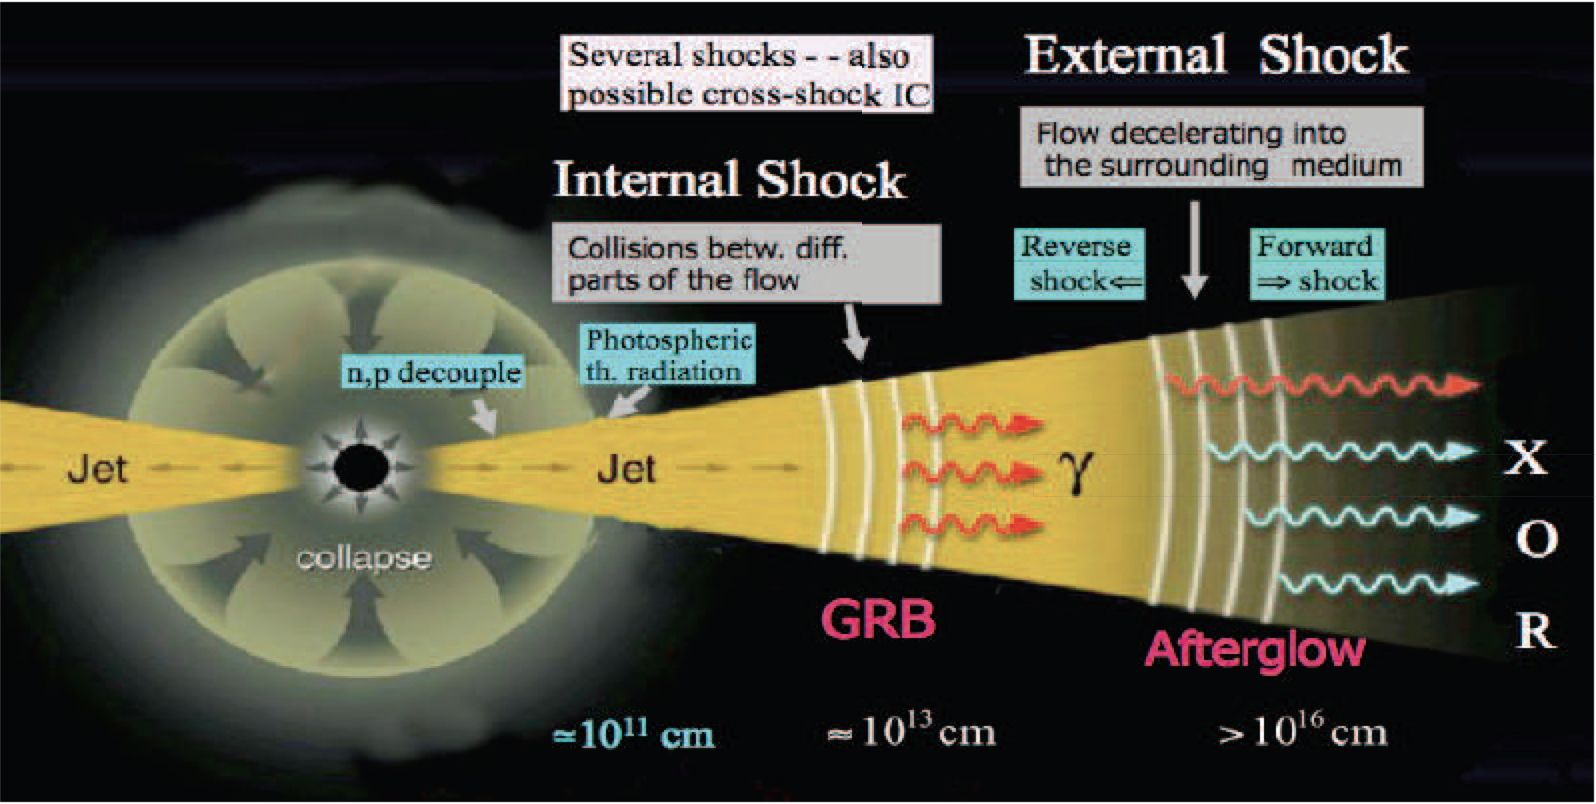
\includegraphics[width=\textwidth]{gfx/grbmec}
	
	\caption{Schematic view of the emission mechanisms in the traditional fireball
model. Schematic taken from \citet{Meszaros2014}.}
	
	\label{fig:intro:grbglow}
\end{figure}

Because the explosion mechanism itself is hidden from sight inside the exploding
star, direct detection of the collapse is extremely difficult if not impossible. The prompt
emission is in
many cases too short for detailed investigation so an informative
way to learn
about the GRB explosion mechanism is to investigate the afterglow,
which is
visible for longer periods of time, allowing for ground based
follow-up. Because
the afterglow is a featureless power-law continuum in the optical \citep{Paradijs2000},
just as with the
quasar continuum, it can be used to infer the properties of the
intervening material, both
in the host galaxy and in potential DLA systems.
Since the sight-lines selected
by GRB afterglow are different than the ones
selected by quasars, they provide
an independent view of otherwise unobservable
galaxies. Since the
quasars are always positioned in the center of the host
galaxies and the
long GRBs are shown to trace the stellar light
\citep{Fruchter2006,
Anderson2015}, this potentially could make a difference in
the picture drawn by using the two types of phenomena.
Additionally, since GRBs are visible to such extreme
redshifts
\citep[8.2 and 8.1,][]{Tanvir2009, Salvaterra2009}, they provide a
unique probe to trace star formation at
the earliest times. 

A ground-based follow-up program has been undertaken using X-shooter, in which
all \textit{Swift}-bursts with galactic A$_{V} \leq 0.5$ and an XRT position
within 10 minutes are followed up, if possible. This program has led to a lot of
papers, investigating single bursts \citep[e.g.][to mention some]{Sparre2011,
DElia2014, Kruhler2013a, Xu2013a, DeUgartePostigo2014, Schulze2014a, Japelj2015,
Hartoog2015} which include GRBs with identified associated SNe, short GRBs and
detections of molecular hydrogen. 
In Paper III \citep{Japelj2015} we
investigate the shape of the extinction curves in the host
galaxies, at the
position of the GRBs, for a sample of extincted afterglows. An
example of an
extincted afterglow is shown in Fig.\,\ref{fig:intro:grbext} where
the spectrum
is shown in black and the continuum level estimation shown in red.
From the
normalized spectrum the neutral hydrogen column density can be
estimated and
from the modeling the afterglow SED the preferred extinction law
can be
inferred. For the sample of eight bursts we investigated here, there
seemed to
be a preference for SMC-like dust towards the GRB sightlines. 

\begin{figure}[htb]
	
	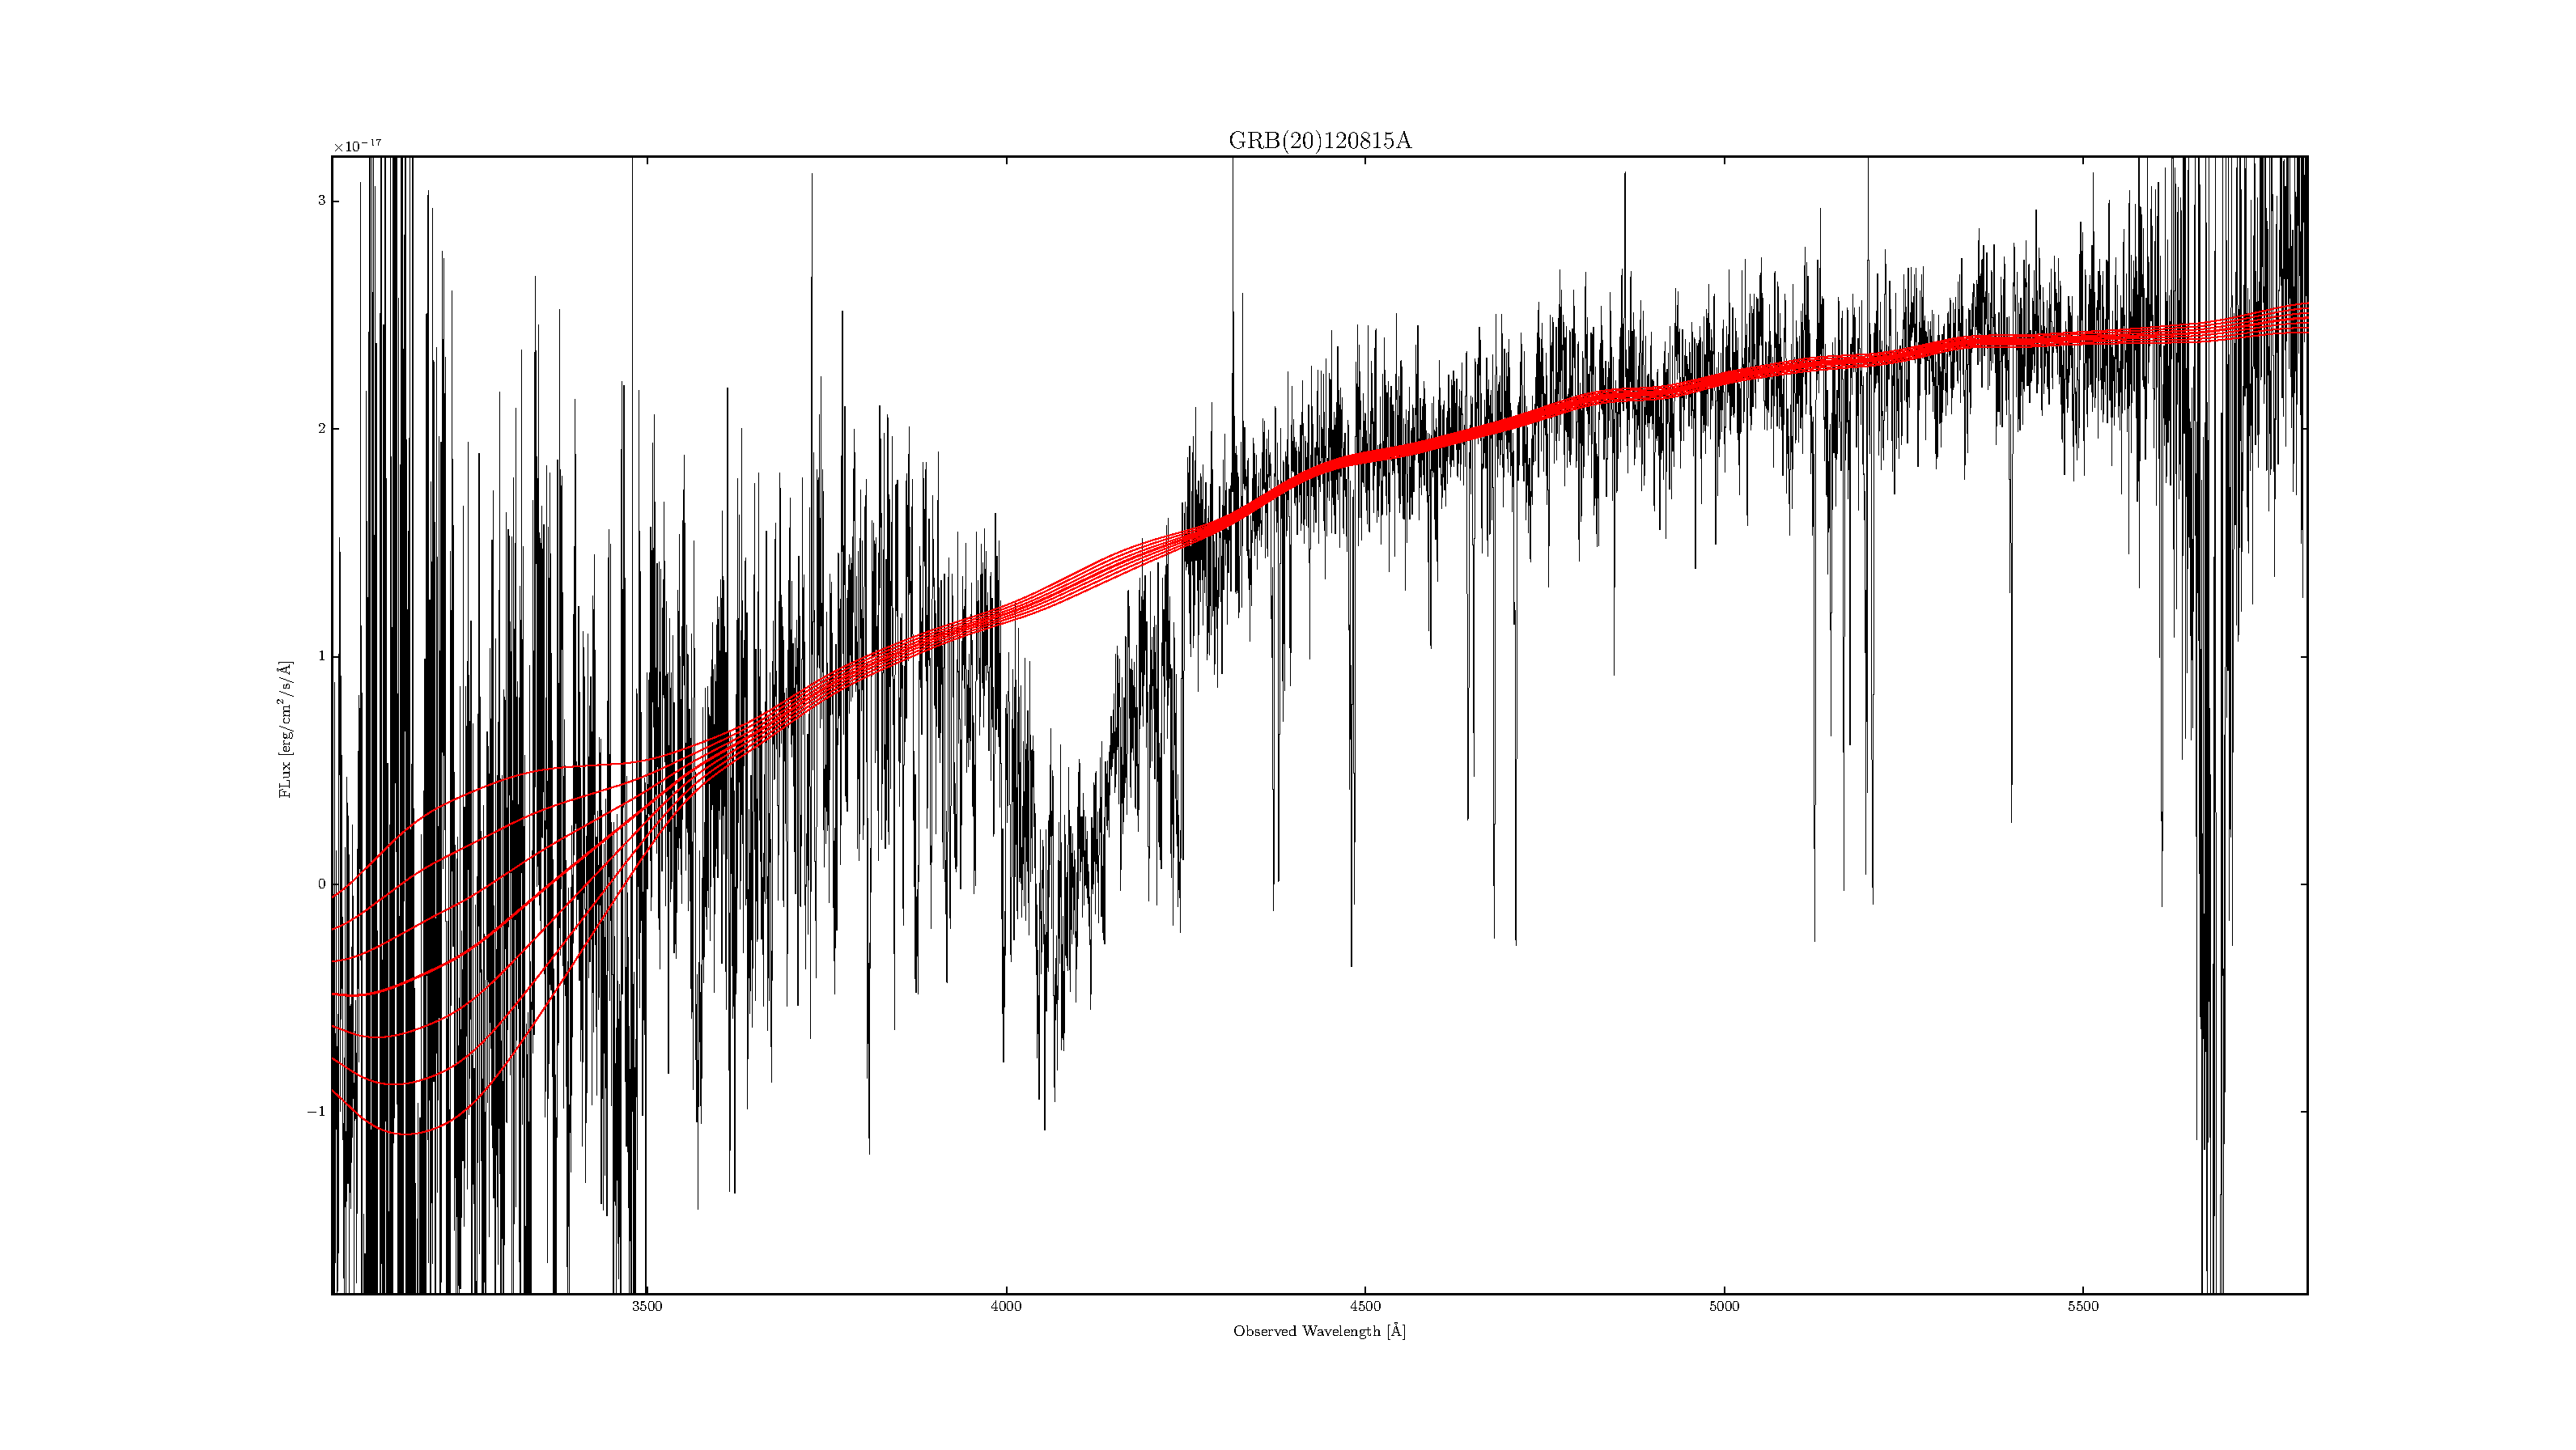
\includegraphics[width=\textwidth]{gfx/normspec}
	
	\caption{Extincted afterglow spectrum of GRB\,120815A in black. The broad
absorption feature at 4100 \AA~ is from Lyman $\alpha$ absorption in the host
indicating a redshift of $z \sim 2.35$. A multitude of narrow absorption lines
are visible in the spectrum belonging to various ionic species of elements. The
thick red line is the continuum level, as determined from the normalization
algorithm developed, the narrow red lines are the 1, 2, 3 $\sigma$ lines
indicating the uncertainty in the continuum placement. The continuum-level
algorithm I developed will be presented in a future paper.}
	\label{fig:intro:grbext}
\end{figure}

Additionally, for some of the triggers we have executed, only emission from
the
GRB host galaxy is visible. The study of the host galaxies of GRBs in emission
is an
indirect way of investigating whether GRBs prefer unusual environments and
if
the GRBs trace star formation. For a sample of 96 host galaxies, we have
investigated in paper IV \citep{Kruhler2015} whether there is a preference for
GRBs to occur in metal-poor hosts as is expected from the theoretical explosion
models \citep{Woosley1993}. If this is the case, this would mean that GRBs
cannot be used as a
representative proxy for star formation at high redshift and
would have a bias
towards low metallicity environments. What we showed in paper
IV is that there
is indeed a preference for low metallicity host, but only at
low redshift which
is attributed to the metallicity evolution of the universe
where conversely at
redshift $z \sim 3$ most of the star formation in the
universe takes place in
$Z_\odot \leq 0.5$ galaxies and thus the bias of GRB
host towards lower
metallicities disappears.


\section{Supernovae: The fiery deaths of massive stars and their environments.}
\label{sec:intro:sn}
Supernovae are a special class of celestial phenomena related to the death of
heavy stars and has been known since \textit{De stella nova}, published by Tycho Brahe in 1573.
Broadly speaking,
there exists two kinds of SN explosions: thermonuclear and
core-collapse. A
thermonuclear SNe, called type Ia SN, begins with a
carbon-oxygen white dwarf
 gravitationally sustained by electron degeneracy
pressure. The explosion is
started by a potential binary companion transferring
mass via Roche-lobe
overflow, which cause the white dwarf to exceed the
Chandrasekhar mass where
carbon starts to fuse. Because the star is
gravitationally sustained by
degeneracy pressure, the star is isothermal and
when the critical fusion
temperature is reached, the entire star undergoes
runaway thermonuclear
explosion. In the other type of SNe, called SN type II or
core-collapse SN, a
stellar iron core that exceeds the Chandrasekhar limit
undergoes collapse. The Chandrasekhar limit is the maximal mass a
gravitationally bound object, supported by electron degeneracy pressure, can
have. As the density increase during the collapse, electrons will start
being
captured by protons and this speeds up the process by reduction of the
electron degeneracy pressure and the gas pressure. Depending on the initial
properties
of the collapsing star, different scenarios can occur where in some
cases a
compact remnant is left behind, either a neutron star or a black hole.
The
energy from the core-collapse is converted into kinetic energy of the outer
layers, which then decays radioactively, powering the SN.
GRBs and different
kinds of core-collapse SN, are linked to the
deaths of massive stars. However,
neither the progenitor system nor
  the production conditions that lead to each
kind of explosion in a
  massive stripped star are well understood. The
different kinds of
  SNe are determined by the initial mass and metallicity
of
the stellar progenitor, as well as by the metallicity-dependent
mass loss in the
stellar winds at the end phase of their evolution
and the interaction with a
sufficiently close companion star. The rotation of the stellar progenitor may
also be another factor that determines the type of SN explosion. Type Ic SNe are
explosions from the most heavily stripped
  massive stars that have been removed
of both their H and He layers. Long duration gamma-ray bursts (GRBs) may be the
most
extreme cases of stellar explosions, and a few cases have been associated
with broad-lined Type Ic SN \citep{Woosley2006} which is a sub-class of SNe
which resembles type Ic SNe, but has extremely broad lines, indicative of
high-velocity ejecta. Other long GRBs
  surprisingly lacked the distinct SN
signatures \citep{Fynbo2006}. The connection between long-duration GRBs and
broad-lined SNe Ic (SNe Ic-BL/hypernovae) and the existence of SNe Ic-BL without
observed
GRBs raises the question of what distinguishes a GRB progenitor from
that of an ordinary SN Ic-BL without a GRB. This question may be answered by
observing the stellar progenitors, which give rise to
  the various types of SN
explosions. However, searches for SN
  progenitors of type Ibc in images taken
before the explosions have failed,
  because the galaxies are distant and
individual stars are difficult
  to distinguish \citep{Maund2005}. Progenitors
of a few type II SNe has been detected in pre-explosion images \cite{VanDyk2012}
and confirms the massive progenitor scenarios suggested by the models. 

An indirect method to distinguish between the different progenitor scenarios is
to explore the environments at
the locations of the SN and GRBs to look for
systematic trends \citep{Levesque2014}. SN
Ic-BL without observed GRBs lie in
systematically more metal rich
environments than SNe with GRBs
\citep{Modjaz2008, Graham2013}. Integral field data of the host
of
GRB\,980425/SN\,1998bw show that the location of the SN (a Type
Ic-BL) is close
to a very metal poor region, but that the metallicity
variations in HII regions
in the dwarf galaxy host are otherwise minor
\citep{Christensen2008}.  In
comparison, Type Ic sites are shown to be relative
metal rich. Recently the
abundances at the sites of different kinds of
core collapse SNe have been
determined and shows that SNe Type Ic lie
in systematically more metal rich
environments than other types of
core collapse explosions \citep{Modjaz2011,
Leloudas2011, Kuncarayakti2013a, Kelly2012}.  In contrast \citet{Anderson2010}
argue
that metallicity is not the dominant parameter for the SN type. The
metallicity difference may have a physical origin, as a higher
metallicity may
give rise to stronger line-driven winds that remove
the outer H and He layers of
the star \cite{Vink2005}, a necessary condition for
a Type Ic SNe. This argument
does not explain the lower abundances at
the sites of SNe Ic-BL as well as at
GRB regions, since GRB
progenitors are expected to be metal poor
\citep{Woosley1993}, unless the GRB-SN
progenitors underwent a peculiar
evolutionary phase marked by chemical
homogeneous mixing. A possible solution to
this dilemma is a massive
binary progenitor system, rather than a metallicity
effect.

Using integrated central oxygen abundance of the host
galaxy as a proxy for the
SN site \citep{Prieto2008, Kelly2012}, adopting the
luminosity-metallicity
relation for SDSS galaxies \citep{Tremonti2004}, gives
systematically larger
abundances than those measured in the SNe regions \citep{Modjaz2011}.
This
offset is not surprising since galaxies targeted for SNe searches
are more
luminous and massive and consequently have higher abundances
and they can have
abundance gradients in their disks \citep{Sanders2012}.
% Modjaz et al. include
%SNe found in both targeted surveys and
% serendipitously detected SNe. 
%although including both targeted and non
%targeted galaxies should mitigate
%systematic effects.
To understand SN progenitors it is important to establish
the
systematic effects, which arise from the oxygen abundance
determinations,
when only an integrated spectrum can be obtained
(e.g. low-luminosity or
distant, unresolved galaxies), as well as the
implications of metallicity
gradients in large massive galaxies.

To try and answer the question about what determines the type of SN Ic
exploding, we have taken data for 19 SN Ic and Ic-BL hosts using the IFU
installed at VLT/VIMOS which gives spatially resolved spectra allowing
diagnostics
to be determined locally which for the redshift of the host
corresponds to the
physical sizes of the molecular clouds hosting the stellar
progenitor
population. We show in Fig.\,\ref{fig:intro:snifu} a mosaic of the
H$\alpha$
emission determined from the VIMOS data superposed on the SDSS images
of the
host which we can translate into a star formation rate. Additionally
using
stellar population modeling, we can constrain the progenitor age and
thereby the
mass that will help discerning between the different types of
progenitor stars. 



\begin{figure}[htb]
	
	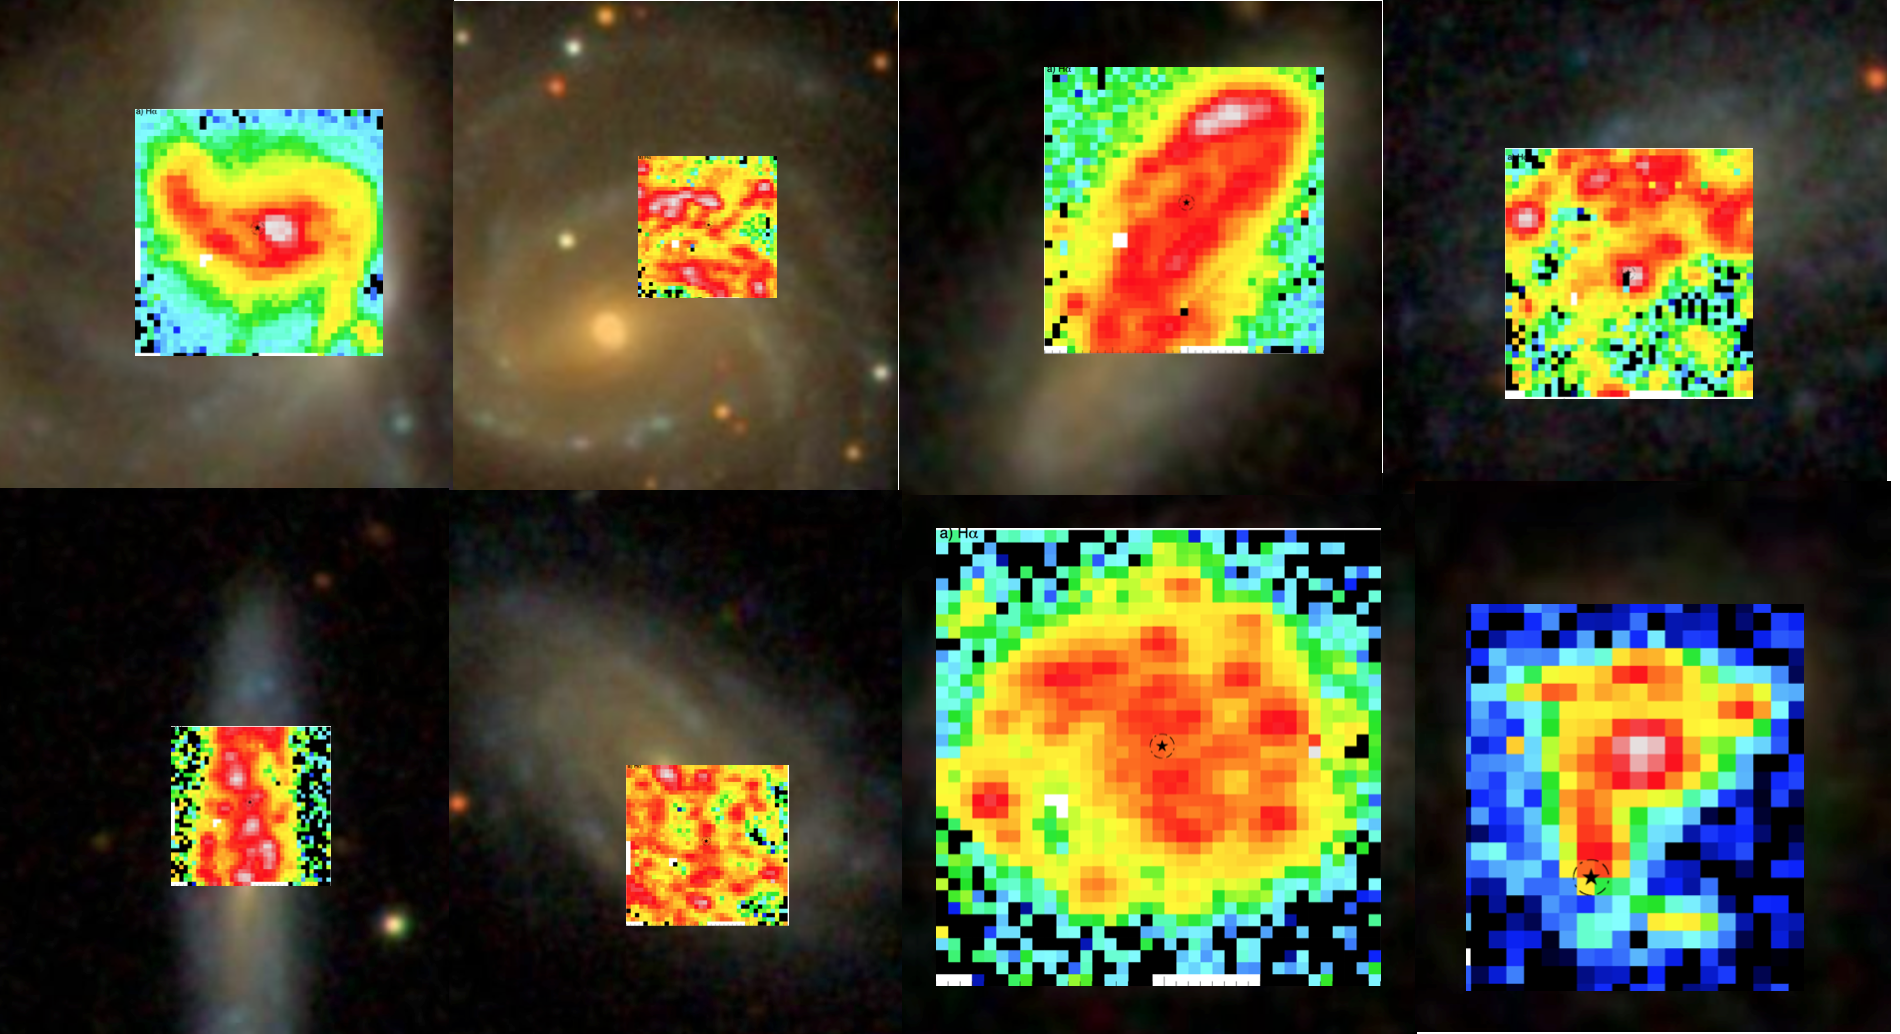
\includegraphics[width=\textwidth]{gfx/ifu}
	
	\caption{A mosaic showing 8 of the targeted SN Ic and Ic -BL host galaxies with the H$\alpha$ flux determined from the VIMOS observation superposed on the SDSS postage stamps. This is part of our sample, investigating the local properties of helium-poor SNe. }
	
	\label{fig:intro:snifu}
\end{figure}

For the metallicities determined locally we reproduce the trend seen earlier
that Ic-BL prefer lower metallicity environments as compared to normal Ic, which
we show in Fig.\,\ref{fig:intro:snmet}. This is still preliminary very work
and the values might chance slightly. A thing to note is that the 1-$\sigma$
intervals around the mean values are consistent within the errors, therefore
pointing to a non-significant difference in the types of environments preferred.



\begin{figure}[htb]
	
	\includegraphics[width=\textwidth]{gfx/snmet}
	
	\caption{Number of SNe as a function of metallicity. The green colors represent the metallicity if SN Ic-BL and the blue represent the metallicity of SN Ic. A marginal evidence for a preference for lower-metallicity environments is shown.}
	
	\label{fig:intro:snmet}
\end{figure}

An additional project we have been working on is the detection and follow-up of
magnified SNe in the Frontier Fields.
Over the past decade, the deep HST
Treasury surveys (GOODS, CANDELS, CLASH) have
enabled "free" SN searches, which
have collectively
accumulated scores of SN detections that reach to uniquely
high redshifts
\citep{Riess2007, Rodney2014b, Graur2014} in clusters of galaxies
selected for observations over large periods of time with relatively high
cadence.

The ongoing Hubble Frontier Fields program now provides a powerful new tool for
the discovery of
particularly high-z SNe. Gravitational lensing in the prime
fields can
magnify fluxes significantly, making it possible to detect distant
background
events. 
The Hubble Frontier Field survey thus provides the first
opportunity to discover
SNe at 2 < z < 3, building up a small but important “New
Frontier” sample.
Because Type Ia SNe are standardizable candles as a
consequence of the similar ejected Ni$^{56}$-masses, we can use lensed SNe Ia to
directly measure the true lensing magnification $\mu$ and confront the
predictions from existing lens models \citep[e.g.][]{Riehm2011, Li2012,
Patel2014}. Our sample of lensed SNe Ia is already proving
to be a very valuable
tool for testing galaxy cluster dark matter models \citep{Rodney2015}, which
will be particularly valuable for the study of z > 8 galaxies magnified by these
clusters \citep[e.g.][]{Zheng2012}.



The unique combination of deep imaging, strong lensing, and rapid cadence in the
HFF program has also provided two very exciting discoveries of multiply-imaged
transients. In January and August of 2014, we observed two short transient
events in separate images of the same strongly lensed galaxy, measured to be at
z=1.005 with X-shooter. Collectively nicknamed “Spock”, both
of these events are
too faint to be a normal SN and too bright to be a stellar
flare. The light
curves are also faster than expected from a He shell explosion
on a white dwarf
\citep[a “.Ia” event][]{Bildsten2007}, and fainter than any of
the “fast optical
transients” yet seen in wide-field ground-based surveys
\citep[e.g.][]{Kasliwal2010, Poznanski2010a, Vinko2014}.
Lens models (and
Occam’s razor) suggest that these two events are most likely
spatially
coincident on the source plane. If the two events were also coincident
in time,
then this could be an example of an extremely rare neutron star
collision
\citep[a “kilonova”][]{Tanvir2013, Barnes2013}. If not, these may be
two
separate outbursts from an extremely bright nova with a remarkably fast
recurrence timescale of $\sim$1 year. This would be a unique nova, as it would
have a recurrence timescale on par with the most extreme examples known
\citep{Tang2014} and would also be at least an order of magnitude more luminous
than a typical nova.
In November of 2014 we discovered another exciting
transient, this time with
four distinct sources appearing almost simultaneously
in a strongly lensed
spiral galaxy at z = 1.5. Dubbed “SN Refsdal,” this is the
first ever example of
a strongly lensed SN with multiple resolved images
\citep[][Figure
3]{Kelly2014}. The Einstein Cross configuration is generated by
a galaxy-scale
lens, but the SN host galaxy is also multiply imaged by the
cluster, so we
expect to see SN Refsdal return elsewhere in the cluster field in
1–5 years
\citep{Oguri2015, Sharon2015}. Measurements of the relative
magnifications and
time delays among these multiple images will soon deliver an
unprecedented suite
of powerful new mass model constraints and the reappearance
of "SN Refsdal" in the future will be a crucial test for these mass models. 

With the X-shooter observations we have obtained of "SN Refsdal" in paper II, we
see a clear
detection of a broad H$\alpha$ at a redshift consistent with the
host galaxy,
which we show in Fig.\,\ref{fig:intro:snref}. By matching templates
to the
spectrum of "SN Refsdal" we confirm that the best matching existing SN
spectra
is similar to that of the peculiar type II SN, SN 1987A.
 


\begin{figure}[htb]
	
	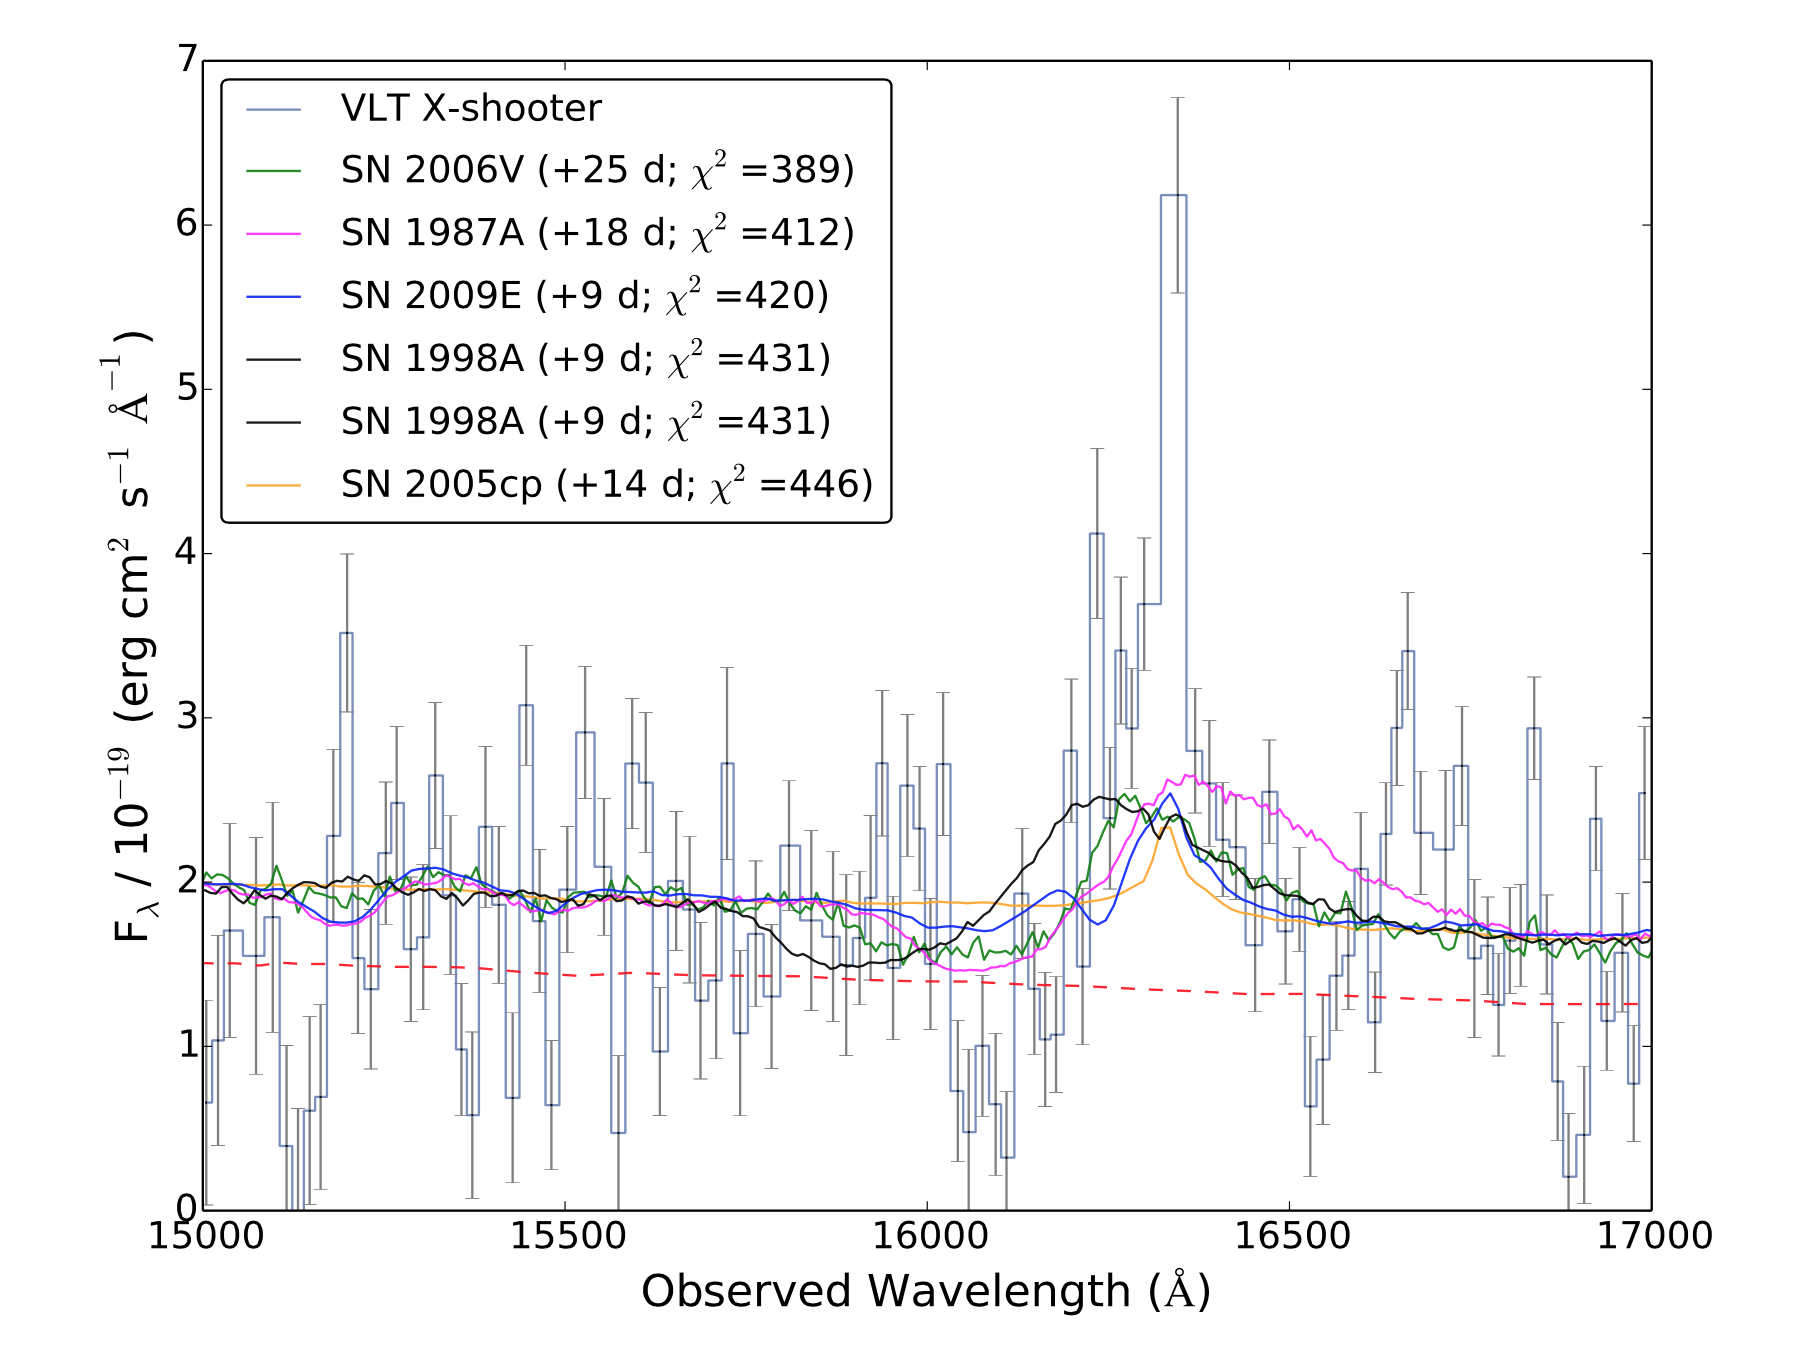
\includegraphics[width=\textwidth]{gfx/SNref}
	
	\caption{X-shooter spectrum of the quadruply lensed SN, Refsdal. The broad feature at 16300 \AA~is H$\alpha$-emission from the SN explosion. Over plotted are the best fit templates.}
	\label{fig:intro:snref}
\end{figure}

\clearpage

\section{Future work}
\label{sec:intro:fut}

Having just started my scientific change of environment at UCSC, I will work
with Enrico Ramirez-Ruiz on a project related to the explosions of SNe,
specifically how the polarization of the elements synthesized in the explosion
depends on the regions in which they are deposited. Additionally I will work on
a project with Jason Xavier Prochaska related to my work on quasars. 
The "SN
Refsdal" classification-paper is nearing progressing and during my stay
in
California, I will visit Patrick Kelly at Berkeley to collaborate on
finishing
it. My VIMOS project is quite progressed and I have begun drafting a
paper,
which I hope to finish within the next year. Additional work is needed for
the
population fitting and this will likely require a great deal of time to  do.
As
the X-shooter afterglow sample continues to grow, I will normalize the
spectra
as they are delivered and when I return from my exchange, produce the X-shooter
afterglow composite for which I will write a paper, similar to the quasar paper.

I have finished all of my mandatory duties in teaching and courses, so I can
devout the entire last two years of my PhD studies on doing research, which I
look forward to.


\section{Acknowledgments}
I would first and foremost like to thank my supervisor, Lise Christensen for
making this work possible. Johan Fynbo has been great when is comes to the
quasar projects and Jens Hjorth has been awesome when it comes to the SN work.
Marianne Vestergaard is always great to discuss all things AGN with. I would
like to thank all of my great colleagues at DARK for making the first two years
of my PhD-studies very enjoyable.


 % INCLUDE: introduction
%% !TEX root = ../thesis-example.tex
%
\chapter{Related Work}
\label{sec:related}

\cleanchapterquote{A picture is worth a thousand words. An interface is worth a thousand pictures.}{Ben Shneiderman}{(Professor for Computer Science)}

\Blindtext[2][1]

\section{Related Work Section 1}
\label{sec:related:sec1}

\Blindtext[2][2]

\section{Related Work Section 2}
\label{sec:related:sec2}

\Blindtext[3][2]

\section{Related Work Section 3}
\label{sec:related:sec3}

\Blindtext[4][2]

\section{Conclusion}
\label{sec:related:conclusion}

\Blindtext[2][1]
 % INCLUDE: related work
%% !TEX root = ../thesis-example.tex
%
\chapter{System}
\label{sec:system}

\cleanchapterquote{Innovation distinguishes between a leader and a follower.}{Steve Jobs}{(CEO Apple Inc.)}

\Blindtext[2][1]

\section{System Section 1}
\label{sec:system:sec1}

\Blindtext[1][2]

\begin{figure}[htb]
	\includegraphics[width=\textwidth]{gfx/Clean-Thesis-Figure}
	\caption{Figure example: \textit{(a)} example part one, \textit{(c)} example part two; \textit{(c)} example part three}
	\label{fig:system:example1}
\end{figure}

\Blindtext[1][2]

\section{System Section 2}
\label{sec:system:sec2}

\Blindtext[1][2]

\begin{figure}[htb]
	\includegraphics[width=\textwidth]{gfx/Clean-Thesis-Figure}
	\caption{Another Figure example: \textit{(a)} example part one, \textit{(c)} example part two; \textit{(c)} example part three}
	\label{fig:system:example2}
\end{figure}

\Blindtext[2][2]

\section{System Section 3}
\label{sec:system:sec3}

\Blindtext[4][2]

\section{Conclusion}
\label{sec:system:conclusion}

\Blindtext[2][1]
	% INCLUDE: system
%% !TEX root = ../thesis-example.tex
%
\chapter{Concepts: This text is here to test a very long title, to simulate the line break behavior, to show that an extremely long tilte also works}
\label{sec:concepts}

\cleanchapterquote{Users do not care about what is inside the box, as long as the box does what they need done.}{Jef Raskin}{about Human Computer Interfaces}

\Blindtext[2][1]

\section{Concepts Section 1}
\label{sec:concepts:sec1}

\Blindtext[2][2]

\section{Concepts Section 2}
\label{sec:concepts:sec2}

\Blindtext[3][2]

\section{Concepts Section 3}
\label{sec:concepts:sec3}

\Blindtext[4][2]

\section{Conclusion}
\label{sec:concepts:conclusion}

\Blindtext[2][1]
 % INCLUDE: concepts
% !TEX root = ../thesis-example.tex
%
\chapter{Conclusion}
\label{sec:conclusion}

\Blindtext[2][1]

\section{System Section 1}
\label{sec:conclusion:sec1}

\Blindtext[2][2]

\section{System Section 2}
\label{sec:conclusion:sec2}

\Blindtext[3][2]

\section{Future Work}
\label{sec:conclusion:future}

\Blindtext[2][2]
 % INCLUDE: conclusion
%\cleardoublepage

% --------------------------
% Back matter
% --------------------------
{%
\setstretch{1.1}
\renewcommand{\bibfont}{\normalfont\small}
\setlength{\biblabelsep}{0pt}
\setlength{\bibitemsep}{0.5\baselineskip plus 0.5\baselineskip}



\printbibliography[nottype=online]
%\printbibliography[heading=subbibliography,title={Webseiten},type=online,prefixnumbers={@}]
}

%\cleardoublepage

\listoffigures
%\cleardoublepage

\listoftables
%\cleardoublepage

% !TEX root = ../thesis-example.tex
%
\pagestyle{empty}
\hfill
\vfill
\pdfbookmark[0]{Colophon}{Colophon}
\section*{Colophon}

This thesis was typeset with \LaTeXe.
It uses the \textit{Clean Thesis} style developed by Ricardo Langner.
The design of the \textit{Clean Thesis} style is inspired by user guide documents from Apple Inc.

Download the \textit{Clean Thesis} style at \url{http://cleanthesis.der-ric.de/}.

%\cleardoublepage

% !TEX root = ../thesis-example.tex
%
%************************************************
% Declaration
%************************************************
\pdfbookmark[0]{Declaration}{Declaration}
\chapter*{Declaration}
\label{sec:declaration}
\thispagestyle{empty}

You can put your declaration here, to declare that you have completed your work solely and only with the help of the references you mentioned.

\bigskip

\noindent\textit{\thesisUniversityCity, \thesisDate}

\smallskip

\begin{flushright}
	\begin{minipage}{5cm}
		\rule{\textwidth}{1pt}
		\centering\thesisName
	\end{minipage}
\end{flushright}

%*****************************************
%*****************************************

%\clearpage
%\newpage
\mbox{}

% **************************************************
% End of Document CONTENT
% **************************************************
\end{document}
